\chapter{Opis projektu i jego rozwiązania}
\section{Temat i analiza zadania projektowego}

Zadaniem projektowym jest stworzenie systemu do rozpoznawania cyfr pisanych ręcznie z użyciem sieci MLP. Dane będą pochodzić ze zbioru MNIST.


Dane zadanie jest problemem odpowiedniego przyporządkowania obrazków do odpowiadająych im kategorii na podstawie cyfr tworzonych przez ich piksele. 
Należy więc stworzyć klasyfikator, który poprawnie przydzieli dany obrazek do jednej z 10 klas (każda cyfra z przedziału $0-9$ tworzy jedną klasę).
Zadanie zostanie rozwiązane poprzez stworzenie sieci neuronowej przy pomocy biblioteki TensorFlow.

\section{Techniczne szczegóły zastosowanej sieci}
\subsection{Ogólna struktura sieci}
Zadanie to rozwiążemy stosując sieć neuronową MLP (Multi Layer Perceptron), to jest sieć neuronową typu \textit{feedforward}, zawierającą jedną lub więcej wartw ukrytych sztucznych neuronów. Jej struktura pokazana jest na rys. \ref{netstructure}.
\newline
\begin{center}
	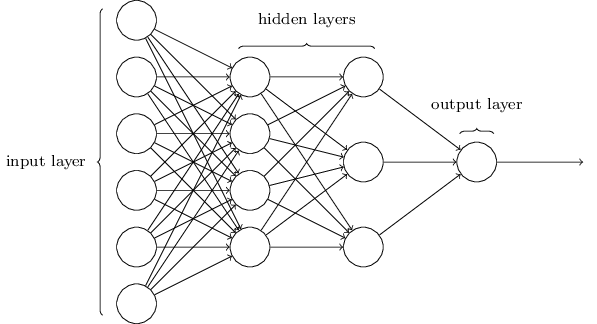
\includegraphics[width=15cm]{utils/tikz11.png}
	\captionof{figure}{Struktura sieci MLP}
	\label{netstructure}
\end{center}

\subsection{Sztuczny neuron}
Pojedynczy neuron pokazany jest na rys. \ref{neuron}. Wykonuje on iloczyn skalarny wektorów tworzonych przez wartości wejść $x_j$ i odpowiadające im wagi $w_j$ po czym dodaje do niego wielkość \textit{bias}:

\begin{equation}
\sum w_jx_j + bias
\end{equation}

Tak otrzymana wartość jest podawana jako argument funkcji wzbudzenia neuronu. Dopiero wynik tej funkcji jest wynikiem końcowym neuronu, \textit{output} na rys. \ref{neuron}.
\newline
\begin{center}
	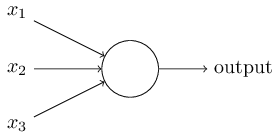
\includegraphics[width=9cm]{utils/neuron.png}
	\captionof{figure}{Pojedyńczy neuron}
	\label{neuron}
\end{center}

\subsection{Funkcja wzbudzenia neuronów}
Zastosowana funkcja wzbudzenia naszej sieci MLP będzie miała postać funkcji sigmoidalnej, przedstawionej na rys. \ref{sigm}.
Funkcja tej postaci zapewnia nam dwie korzyści:

\begin{enumerate}
	
	\item Małe zmiany wejść neuronów będą skutkowały niewielkimi zmianami na wyjściu funkcji sigmoidalnej; pozwoli to kontrolować proces uczenia (w przypadku np. funkcji pobudzenia postaci funkcji skokowej, nawet małe zmiany wejść mogą powodować nieprzewidywalne zachowanie całej sieci);
	\item Funkcja ta jest różniczkowalna, co jest kluczowe w algorytmie uczenia wykorzystującym mechanizm wstecznej propagacji (ang. \textit{backpropagation}).
	
\end{enumerate}
\vspace{1cm}
\begin{center}
	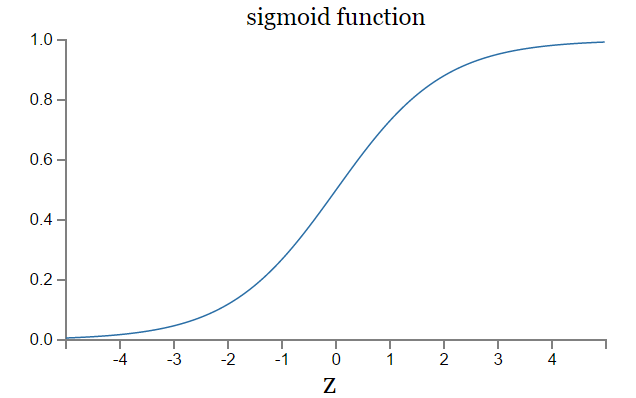
\includegraphics[width=13cm]{utils/sigm.png}
	\captionof{figure}{Postać funkcji sigmoidalnej}
	\label{sigm}
\end{center}


\subsection{Warstwa wejściowa}
Zbiór MNIST składa się z 70,000 obrazków przedstawiających pisane ręcznie cyfry. Każdy z obrazków ma wymiary 28x28, co daje  ilość  $28*28 = 784$ pikseli na każdej ilustracji. Nasza sieć będzie posiadała dokładnie tyle wejść - każdy z neuronów warstwy wejściowej (\textit{input layer} na rys. \ref{netstructure}) będzie otrzymywał dane z jednego i tego samego dla wszystkich danych pikselu obrazka.

\subsection{Warstwa wyjściowa}
Warstwa wyjściowa natomiast (\textit{output layer} na rys. \ref{netstructure}) będzie składała się z 10 neuronów: każdy z nich będzie sygnalizował stopień przynależności obrazka do danej klasy.

Stopień przynależności, jako konsekwencja zastosowania sigmoidalnej funkcji wzbudzeń neuronów, będzie zawierał się w przedziale $<0, 1>$. Największa wartości ze zbioru neuronów wyjściowych będzie wskazywała aktualnie identyfikowaną cyfrę.

\subsection{Proces uczenia}
Do nauki sieci zostanie wykorzystany algorytm wstecznej propagacji (ang. \textit{backpropagation}). Zadanie uczenie sieci przy pomocy tego algorytmu polaga na minimalizacji funckji straty (ang. \textit{loss funtion}) jako funkcji wag i parametrów bias. Funkcja ta została przedstawiona jako wzór  \ref{lossf}, gdzie: $w$ - wagi, $b$ - bias, $n$ - liczebność zbioru uczącego, $y(x)$ - pożądane wyjście dla danego wejścia,  $a$ - rzeczywisty wynik działania sieci dla danego wejścia.

Algorytm ten polega na aplikowaniu do wag drobnych poprawek $\Delta w$ wyliczonych ze wzoru \ref{deltav}, gdzie $ \nabla C$ jest gradientem funkcji strat a $\eta$ jest hiperparametrem wyrażającym wielkość kroku. 

Skrótowo mówiąc, po każdej iteracji, to jest obliczeniu wyniku dla kolejno wszystkich danych uczących, obliczana jest funkcja $C(w,b)$ i jej gradient, a następnie zmieniane są wagi w kierunku przeciwnym do  gradientu funcji strat o krok $\eta$.

\begin{eqnarray}  C(w,b) \equiv
\frac{1}{2n} \sum_x \| y(x) - a\|^2.
\label{lossf}
\end{eqnarray}

\begin{eqnarray}
\Delta w = -\eta \nabla C,
\label{deltav}
\end{eqnarray}


